\documentclass{article}
\usepackage{graphicx}
\usepackage[utf8]{inputenc}
\usepackage[english]{babel}
\usepackage[margin=1.0in]{geometry}
\usepackage{listings}
\usepackage{amssymb}
\usepackage{amsmath}
\usepackage{bbold}
\usepackage{color}
\usepackage{float}
\usepackage{mathtools}
\usepackage{url}
\usepackage[colorlinks,linkcolor = black, urlcolor=black, citecolor =  blue]{hyperref}
\setlength{\parindent}{2em}

\usepackage{algorithm}
\usepackage[noend]{algpseudocode}  %for pseudocode


\begin{document}
\title{Parallelized Conjugate Gradient Solver using MPI and OpenMP }
\author{Timofey Golubev}
\maketitle


\section{Introduction} 
The conjugate gradient (CG) method is an iterative algorithm for numerical solution of systems of linear equations which when written as matrix equations have a symmetric and positive-definite matrix \cite{Golub}. The approach is often used for large matrices where a direct method would take too much time. The solution of the matrix equations is often the most time-consuming portion of a scientific simulation code and often the matrix equations need to be solved many times as part of a self-consistent algorithm \cite{Gummel, Gift}. Therefore, it is very beneficial to apply both shared and distributed memory parallelization techniques \cite{openmp_mpi_paper, mpi_openmp_2}. In this project, I demonstrate use of a hybrid of Message Passage Interface (MPI) (distributed memory) and OpenMP (shared memory) to parallelize this algorithm and study the scaling properties. 

This report is organized as follows. First, the methods used to parallelize the CG algorithm and other technical considerations such as input/output and load balancing are described.  Next, the results including scaling studies, memory usage, effects of different parallelization approaches, and comparisons to Matlab's CG solver are presented and discussed. Finally, I summarize the conclusions and propose ideas for future work.

\section{Methods}

\subsection{Conjugate Gradient Algorithm}
A pseudo-code for the serial CG algorithm for solving the matrix equation $\mathbf{Ax} = \mathbf{b}$ for $\mathbf{x}$, where $\mathbf{A}$ is a symmetric and positive-definite matrix and $\mathbf{b}$ is the right hand side vector is shown below:

\begin{algorithm}
	\begin{algorithmic}[1]
		\caption{Serial Version}
		\State $\mathbf{p} = \mathbf{b}$
		\State $\mathbf{r} = \mathbf{b}$
		\State $\mathbf{x} = \mathbf{x_0}$
		
		\For{$i = 0$ to max\_iter}
		\State $\mathbf{r_{old}} = \mathbf{r}$
		\State $\alpha = \frac{\mathbf{r} \cdot \mathbf{r} }{\mathbf{p} \cdot \mathbf{Ap} }$
		\State //Next estimate of solution:
		\State $\mathbf{x} = \mathbf{x} + \alpha \mathbf{p}$
		\State $\mathbf{r} = \mathbf{r} - \alpha \mathbf{Ap}$
		\State //Check for convergence:
		\If{$\mathbf{r} \cdot \mathbf{r} < $ tolerance}
		\State break
		\EndIf
		\State $\beta = \frac{\mathbf{r} \cdot \mathbf{r}}{\mathbf{r_{old}} \cdot \mathbf{r_{old}}}$
		\State $\mathbf{p} = \mathbf{r} + \beta \mathbf{p}$
		\EndFor
		\State Solution is $\mathbf{x}$	
	\end{algorithmic}
\end{algorithm}

I will omit discussion of the mathematics behind this method since that is beyond the scope of the goals of this project. For more background on the conjugate gradient algorithm, please refer to the references.

\subsection{Parallelizing the CG Algorithm}
The CG algorithm is naturally suited for data-based parallelism which means to divide the data and operations on the data among the MPI ranks and OpenMP threads. The other main type of parallelism would be task-based, meaning to have each processor perform a certain different task. As we can see in the above pseudo-code, (almost) each step depends on the previous step so there is not much opportunity for task-based parallelism. Message Passing Interface (MPI) is used by dividing the matrix and vectors into horizontal slices with each rank being responsible for the calculations involving each slice. Additional parallelism is achieved with OpenMP (omp) by multithreading the \texttt{for} loops for the matrix-vector product ($\mathbf{Ap}$), linear combination of vectors, and dot product calculations. The choice of MPI and OpenMP constructs was made by referring to a Parallel Programming textbook \cite{Eijkhout}. A pseudo-code for parallelized algorithm is below:

\begin{algorithm}
	\begin{algorithmic}[1]
		\caption{Parallel Version}
		\State Divide the matrix and vectors among MPI Ranks
		\State //The portions of matrix and vectors are denoted by \texttt{sub}
		\State $\mathbf{p^{sub}} = \mathbf{b^{sub}}$
		\State $\mathbf{r^{sub}} = \mathbf{b^{sub}}$
		\State $\mathbf{x^{sub}} = \mathbf{x^{sub}_0}$
		
		\For{$i = 0$ to max\_iter}
		\State $\mathbf{r^{sub}_{old}} = \mathbf{r^{sub}}$
		\State $\mathbf{A\_sub\_p} =$ \texttt{mat\_times\_vec}($\mathbf{A^{sub}}$, $\mathbf{p}$)  // \texttt{omp parallel for} and/or \texttt{omp simd} used \\
		\State $\alpha = \frac{\mathbf{r^{sub}} \cdot \mathbf{r^{sub}}}{\mathbf{p^{sub}} \cdot \mathbf{A\_sub\_p} }$  // Dot products use \texttt{MPI\_Allreduce} and \texttt{omp parallel for reduction} \\
		\State //Next estimate of solution:
		\State // Tried \texttt{omp tasks} or \texttt{omp sections} to parallelize the next 2 lines
		\State $\mathbf{x^{sub}} = \mathbf{x^{sub}} + \alpha \mathbf{p^{sub}}$ // \texttt{omp simd} and/or \texttt{omp parallel for}
		\State $\mathbf{r^{sub}} = \mathbf{r^{sub}} - \alpha \mathbf{A^{sub}p^{sub}}$
		\State //Check for convergence:
		\If{$\mathbf{r^{sub}} \cdot \mathbf{r^{sub}} < $ tolerance}
		\State break
		\EndIf
		\State $\beta = \frac{\mathbf{r^{sub}} \cdot \mathbf{r^{sub}}}{\mathbf{r^{sub}_{old}} \cdot \mathbf{r^{sub}_{old}}}$
		\State $\mathbf{p^{sub}} = \mathbf{r^{sub}} + \beta \mathbf{p^{sub}}$ // \texttt{omp simd} and/or \texttt{omp parallel for}
		\State \texttt{MPI\_Allgatherv} of $\mathbf{p^{sub}}$ to $\mathbf{p}$ on all Ranks
		\EndFor
		\State \texttt{MPI\_Gatherv} of $\mathbf{x}^{sub}$ to $\mathbf{x}$ on Rank 0
		\State Solution is $\mathbf{x}$
	\end{algorithmic}
\end{algorithm}

After parallelizing the algorithm, I performed scaling studies using square matrices of various sizes (from 64 to 21952 rows) and varied the number of OpenMP threads and MPI ranks used for each CG run. I chose to use a convergence tolerance of $10^{-8}$ as a good compromise between precision and computational intensity. I attempted different parallelization strategies for lines 8, 14, 15, and 20 with the strategies specified in the comments in Algorithm 2. Some representative results are discussed in Section 3. The specifics of the compilers and libraries used are listed in the Supplementary Material.

\subsection{Load Balancing}
With the data-parallel approach, each rank and thread has an approximately equal amount of data and operations to perform and load balancing is achieved naturally. For the dot products, I chose to use \texttt{MPI\_Allreduce} which helps ensure load balancing by having all ranks perform the reduction. The other option would be to use \texttt{MPI\_Reduce} to reduce to Rank 0 and then have Rank 0 broadcast the scalar result to all ranks. This would disproportionally increase the load on Rank 0 and also result in a needlessly more complicated code. The only exception to load balancing is that Rank 0 gathers the final solution vector at the end of the CG loop. Since this is at the end of the algorithm, this blocking communication does not prevent the other ranks from performing further work since there is no additional work to perform. 

\subsection{Input/Output}
Hierarchical Data Format (HDF5) is a high performance data software library and file format which can store heterogeneous data in compact binary format along with meta-data which describes the structure of the stored data \cite{hdf5}. In this project, HDF5 was used for all input/output (I/O). The input file contains the matrix, right hand side, and initial guess of the solution. Once the CG algorithm is complete, the solution as well as information about the run (i.e. CPU time and number of iterations needed to converge) are written into the input file which now also serves as the output file. In this way, all of the information about a matrix and its solution through the CG method is contained in a single file. 

Portions of the I/O were done in parallel. For example, each MPI rank reads (in parallel with other ranks) only the portion of the matrix ($\mathbf{A^{sub}}$ in Algorithm 2) which it needs for the matrix-vector product. The writing of the solution vector was done by MPI Rank 0 after it performed the verification unit test. The solution vector is relatively small compared to the matrix, so parallel output here is not necessary.


\subsection{Sparse Matrices and Compressed Row Storage}
Sparse-matrices frequently arise in scientific computing. For example, the equations resulting from finite-difference discretization can be written as sparse matrix equations. An example of a sparse matrix structure for the 3D Poisson equation with periodic boundary conditions is shown in Figure \ref{fig:sparse_structure}.

\begin{figure}[H]
	\centering
	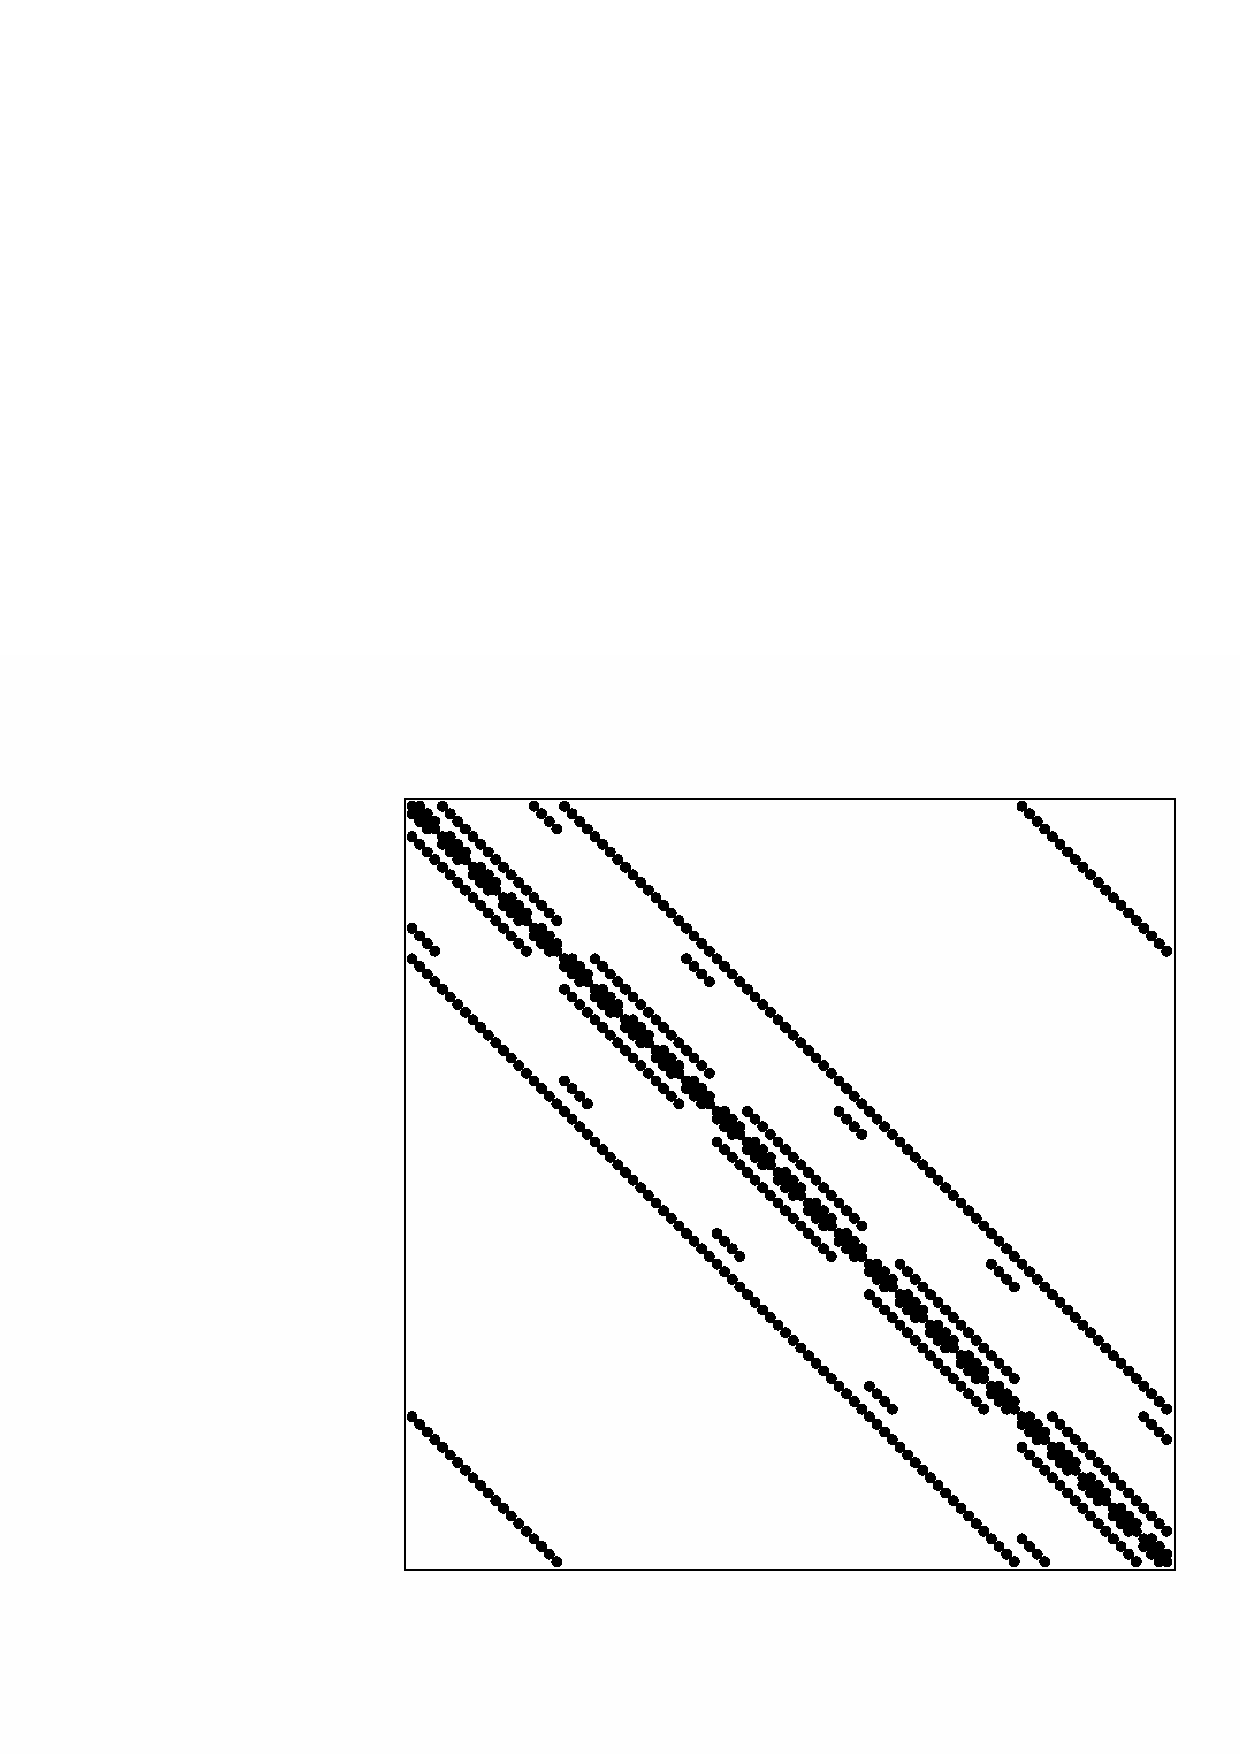
\includegraphics[width=0.8\textwidth]{sparse_poisson_3D_100_2.jpg}  
	
	\caption{Sparse matrix structure for a 100x100 3D Poisson equation with periodic boundary conditions. The circles represent locations of the non-zero elements. This is the matrix structure which is used in the author's solar cell simulation research code.}
	\label{fig:sparse_structure}
\end{figure}

We can take advantage of the sparse property of these matrices to achieve significant performance improvements by storing and operating on only the non-zero elements. One straightforward approach is known as Compressed Row Storage (CRS). In this approach, for each sparse matrix, we store two matrices. One matrix stores all of the non-zero values, while preserving all of the rows (there are generally no empty rows) of the original matrix. The second matrix stores the column indices which describe where the non-zero elements were located in the original matrix. Figure \ref{fig:sparse_to_crs} shows the process of converting a sparse matrix to CRS format.

\begin{figure}[H]
	\centering
    \includegraphics[width=1.0\textwidth]{sparse_to_CRS.jpg}  
	
	\caption{Example of a sparse matrix to compressed row storage conversion.}
	\label{fig:sparse_to_crs}
\end{figure}



\section{Results}
\subsection{Scaling Studies}
We will now describe the results of scaling studies for both dense and sparse matrices. All studies were performed on the High Performance Computing Center at Michigan State University. 

The plots in figure \ref{fig:strong_scaling} shows the speedup for the CG solution of a fixed matrix size relative to a single-threaded run on 1 processor when using multiple MPI ranks and OpenMP threads. The speedup was determined based on an average of several CG solver runs for the same matrix. The different lines represent the strong scaling behavior, while following each individual line represents the thread-to-thread scaling. For dense matrices, we see the best speedup is achieved when using the most MPI ranks and threads. The decrease in speedup for the 4 ranks case when increasing the number of threads to 10 is probably due to too much overhead of creating so many threads without enough work available for each thread to perform in parallel. I expect to see a similar reduction in speedup for the 8 ranks case. 

\begin{figure}[H]
	\begin{minipage}[b]{0.5\linewidth}
		\centering
		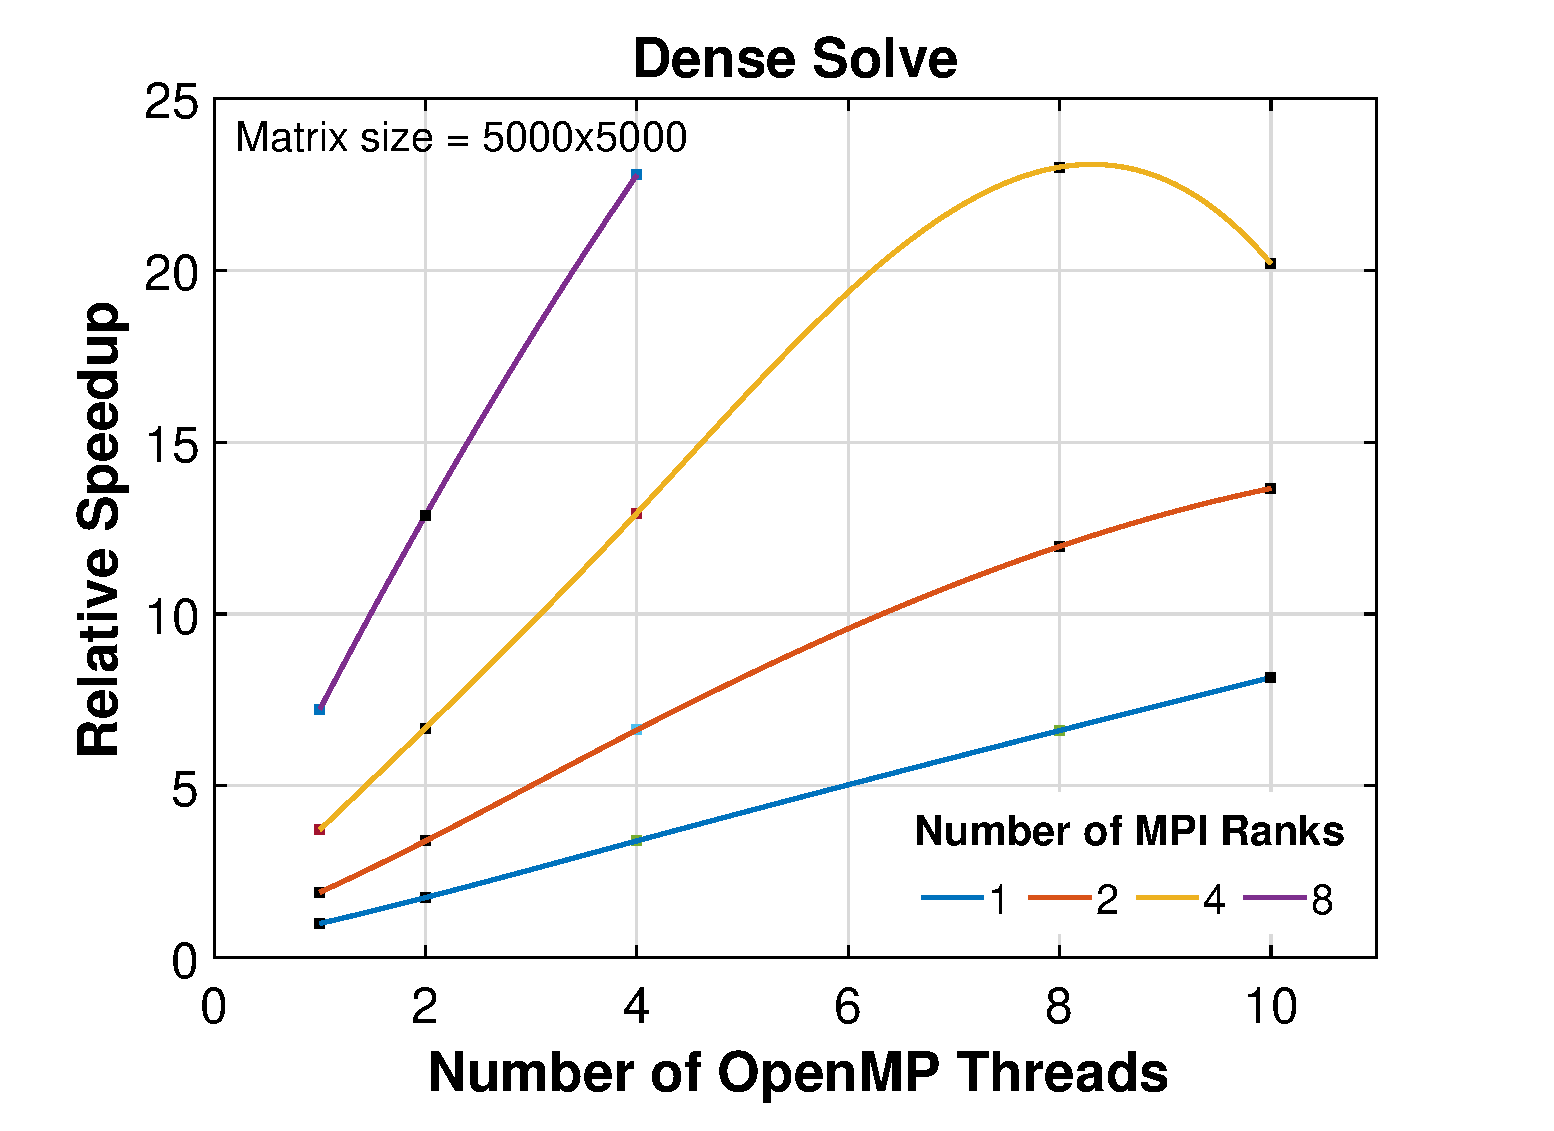
\includegraphics[width=1.0\textwidth]{dense_strong_scaling_report.eps}  
	\end{minipage}
	\begin{minipage}[b]{0.5\linewidth}
		\centering
		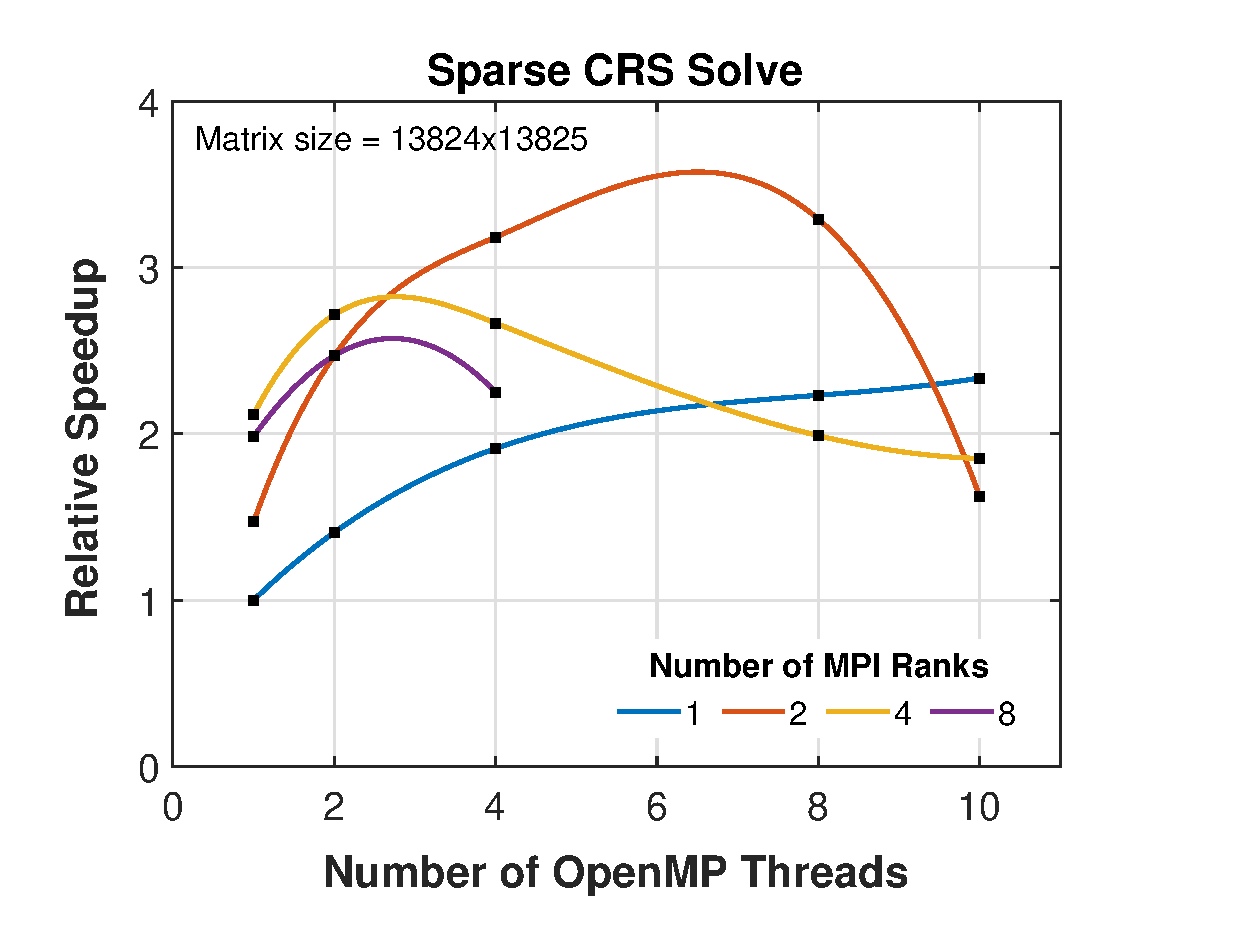
\includegraphics[width=1.0\textwidth]{sparse_strong_scaling_report.eps}  
	\end{minipage}
	\caption{Results of the strong scaling and thread-to-thread scaling studies for dense and sparse matrices. Here the matrix size was fixed while the number of ranks and threads was varied.}
	\label{fig:strong_scaling}
\end{figure}

For sparse matrices, we see a different behavior. The highest speedup was achieved by the two ranks case. The speedup also decreases after a certain thread number threshold and these thresholds are as low as two threads. Only for the single rank case, does the speedup increase with number of threads continuously. Dense matrices have a better scaling behavior than the 3D Poisson equation sparse matrices (stored in CRS format) of similar size. This is most likely due to the drastically higher number of operations needed to be done on a dense matrix than a sparse matrix of the same size. For example, for any sized 3D Poisson equation matrix, after converting to CRS, only 7 columns remain. This means that for a 1000x1000 matrix, instead of having to operate on 1 million elements, with CRS format we only need to operate on 7000. The CPU time is generally at least an order of magnitude less than for the same matrix stored in dense format. There is not much speedup gained when parallelizing small to moderately-sized sparse matrices due to the overhead of MPI message passing and OpenMP thread creation being large relative to the limited amount of operations that need to be done. For large sparse matrices, the scaling behavior becomes more similar to the dense matrix case. In this project, we focus on the small to moderately sized matrices because it is more interesting in terms of understanding parallelization behavior and these are the matrix sizes which I (and probably many others) frequently encounter in research work.

For weak scaling, the matrix size was increased proportionally to the number of MPI Ranks used. Figure \ref{fig:Weak_scaling} shows the weak scaling properties. Here I tested the CPU times for several different OpenMP thread numbers as a function of MPI ranks and problem size (determined by number of elements in the matrix) such that the problem size per MPI ranks remains constant. For the sparse matrices, the problem size was determined after converting the matrices to CRS format. An ideal weak scaling would be flat, showing that the CPU time stays constant as the problem size per rank stays constant. Again we see better scaling behavior for dense matrices, with close to flat curves when 4 or less MPI ranks were used. The CPU time starts increasing when 8 ranks were used probably due to significant overhead in the communication which was not compensated enough by the performance gain of using more ranks. Recall that we have to use \texttt{MPI\_Allreduce} and \texttt{MPI\_Allgatherv} which will result in more communication CPU time with larger problem size even when the number of math operations per rank remains the same. For weak scaling we see increasing CPU times due to the lower amount of operations needed on CRS format matrices causing the speedup from additional parallelization to be not enough to compensate for the increased overhead in communication.


\begin{figure}[H]
	\begin{minipage}[b]{0.5\linewidth}
		\centering
		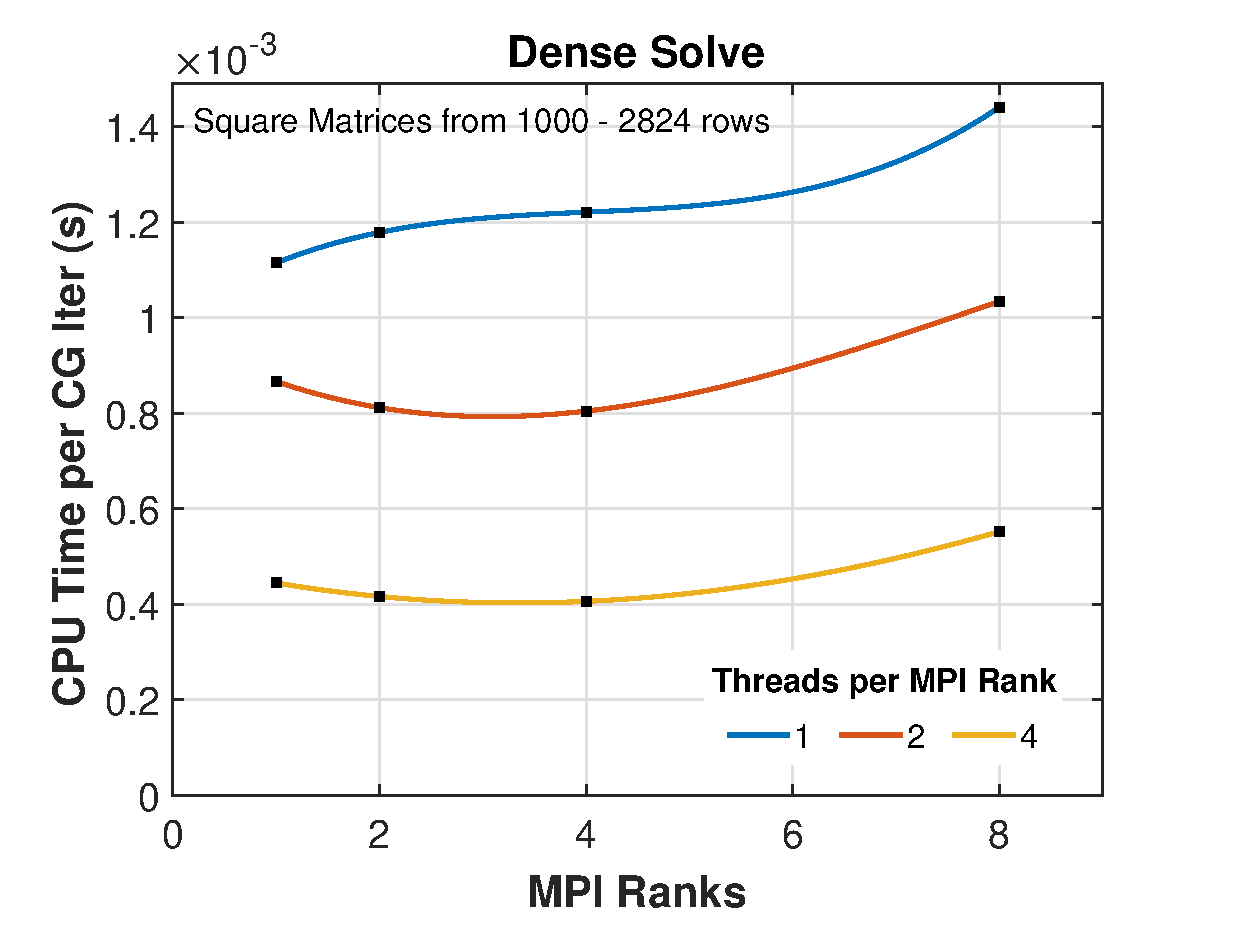
\includegraphics[width=1.0\textwidth]{weak_scaling_dense_report.eps}  
	\end{minipage}
	\begin{minipage}[b]{0.5\linewidth}
		\centering
		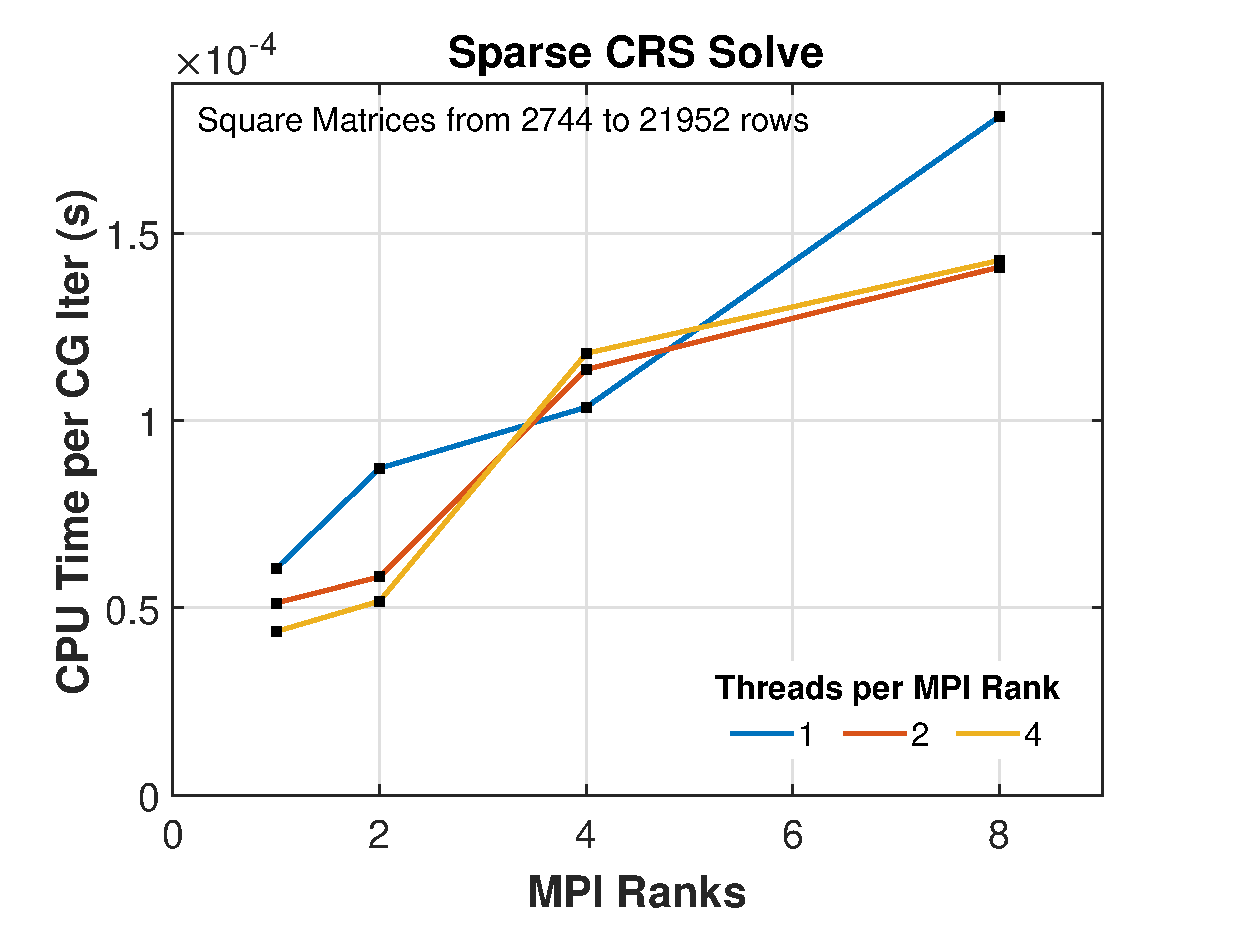
\includegraphics[width=1.0\textwidth]{weak_scaling_sparse_report.eps}  
	\end{minipage}
	\caption{Results of weak scaling studies for both dense and sparse matrices. For weak scaling, the matrix size was increased proportionally to the number of MPI Ranks used.}
	\label{fig:Weak_scaling}
\end{figure}



\subsection{Memory Usage}
Memory usage is optimized through MPI distributed memory parallelization and the data-parallel approach. Each rank is only operating on a sub-block of rows of the matrix and a sub-section of the vectors. This results in a higher likelihood that the data will fit into higher level cache than if we were to operate on the entire matrix and vectors. Also using Compressed Row Storage, highly reduces memory usage for sparse matrices. One way to demonstrate this is to compare the HDF5 file sizes when storing sparse matrices in dense and CRS format (Table \ref{table:file_sizes}). Using CRS format results in significantly smaller file sizes.


\begin{table}[H]
	\centering
	\begin{tabular}{|c|c|c|}
		\hline
		Matrix size & Dense storage file size  & CRS File size  \\
		\hline
		125           &  129 KB  & 20 KB   \\
		1331          &  13.9 MB  &  171 KB   \\
		4913       &  189 MB  & 619 KB  \\
		\hline
		
	\end{tabular}
	\caption{Size of an HDF5 file for storing square matrices (matrix size indicates number of rows=columns) for the 3D Poisson equation using dense vs. CRS format.}
	\label{table:file_sizes}
\end{table} 

\subsection{Effects of different parallelization approaches}
Several alternative approaches to parallelization were attempted. We will discuss these approaches and their effects on the performance. 

One attempt to achieve additional parallelization was to use \texttt{omp tasks} or \texttt{sections} to simultaneously calculate lines 14 and 15 in Algorithm 2. However, this resulted in approximately the same (within statistically reasonable variations) CPU times as the version without the addition of tasks or sections. This is most likely due to the very low computational effort of the linear combinations of vectors in lines 14 and 15 compared to other portions of the code such as the matrix-vector product. Also parallelization with tasks or sections of these 2 lines could at most achieve 2x speedup of that small section of the code and the individual linear combinations were already parallelized by \texttt{omp parallel for reduction}.

Another attempt was to use Single Instruction Multiple Data (SIMD) vectorization either instead, or in combination with \texttt{omp parallel for}. Compilers vectorize loops automatically, but only if a compiler is sure that the data is independent. OpenMP recently introduced the directive \texttt{omp simd} which tells a compiler to vectorize the loop and ignore any doubts about data dependencies. I concentrated on the matrix-vector product function since that is by far the most CPU intensive portion of the algorithm. When replacing the \texttt{omp parallel for} with \texttt{omp simd}, the result was much slower CPU times. The CPU times were actually about the same as for the single-threaded case. \\\\


DESCRIBE THE REASON FOR THIS!!-->  CHECK IF THE NON-SIMD VERSION, HAS THE MAT-VEC PRODUCT LOOP BEING VECTORIZED!!\\\\

It is also possible to combine SIMD vectorization with an OpenMP parallel for loop by using \texttt{omp parallel for simd}. This resulted in the same CPU times as without the vectorization.

\subsection{Verification and Benchmarks}
The correctness of the solver was verified by checking that $\mathbf{Ax} – \mathbf{b} < 10^{-8}$ in a unit test included in the code. The solution results when using different numbers of ranks and threads were also manually checked to ensure that they are nearly the same (to within the chosen tolerance of $10^{-8}$) which is sufficiently accurate for most applications) as the serial case. Results were also cross-checked with Matlab’s CG solver (pcg function). Figure \ref{fig:benchmarks} compares the CPU times of the C++ code with Matlab’s solver. We see that the C++ code is faster than Matlab when using 4 or more MPI ranks. Also, the C++ code has more thread-to-thread speedup on one rank than Matlab. Note that Matlab uses highly optimized Fortran libraries which were developed by large teams of people over many years.

\begin{figure}[H]
	\begin{minipage}[b]{0.5\linewidth}
		\centering
		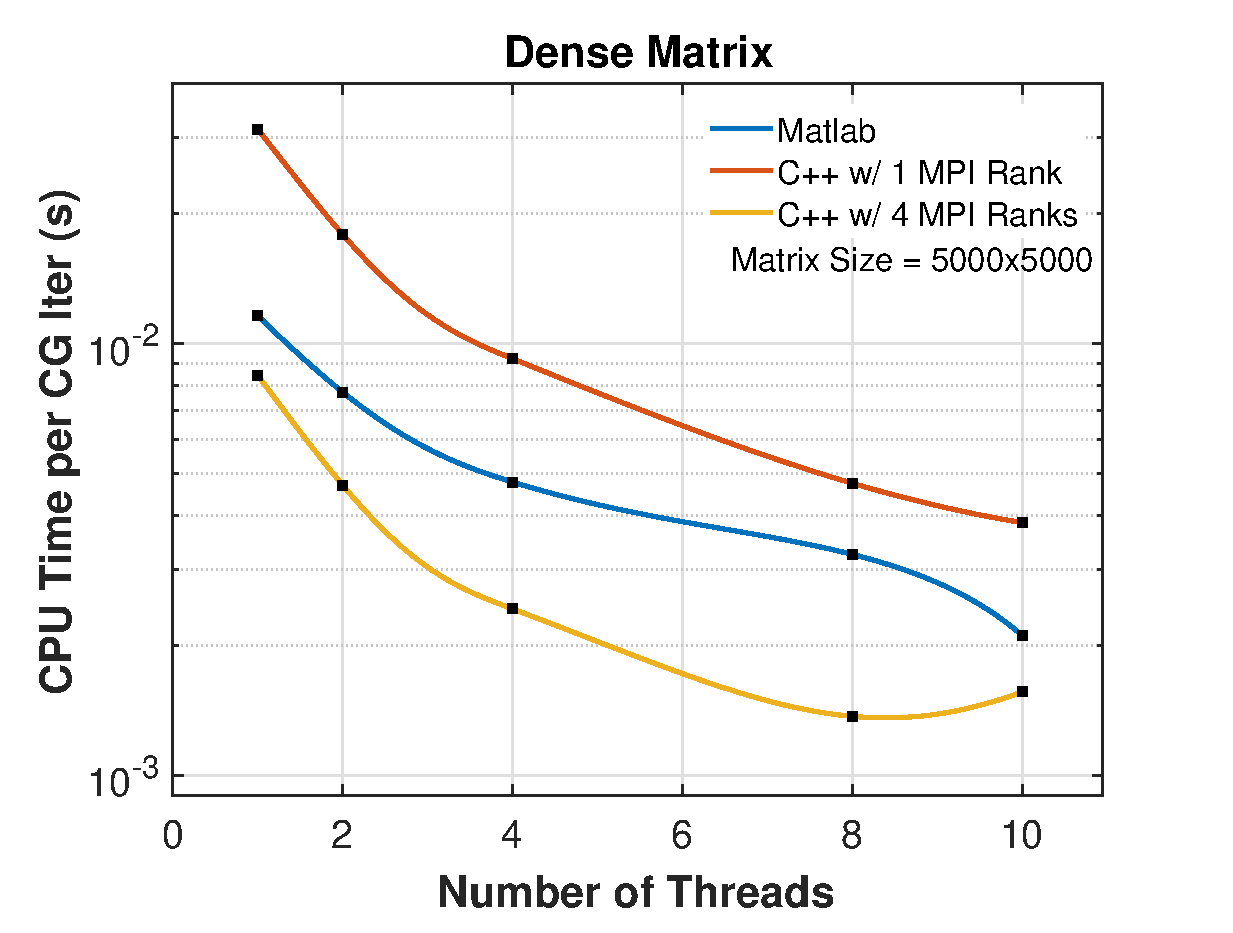
\includegraphics[width=1.0\textwidth]{dense_matrix_benchmarks_log_plot_report.eps}  
	\end{minipage}
	\begin{minipage}[b]{0.5\linewidth}
		\centering
		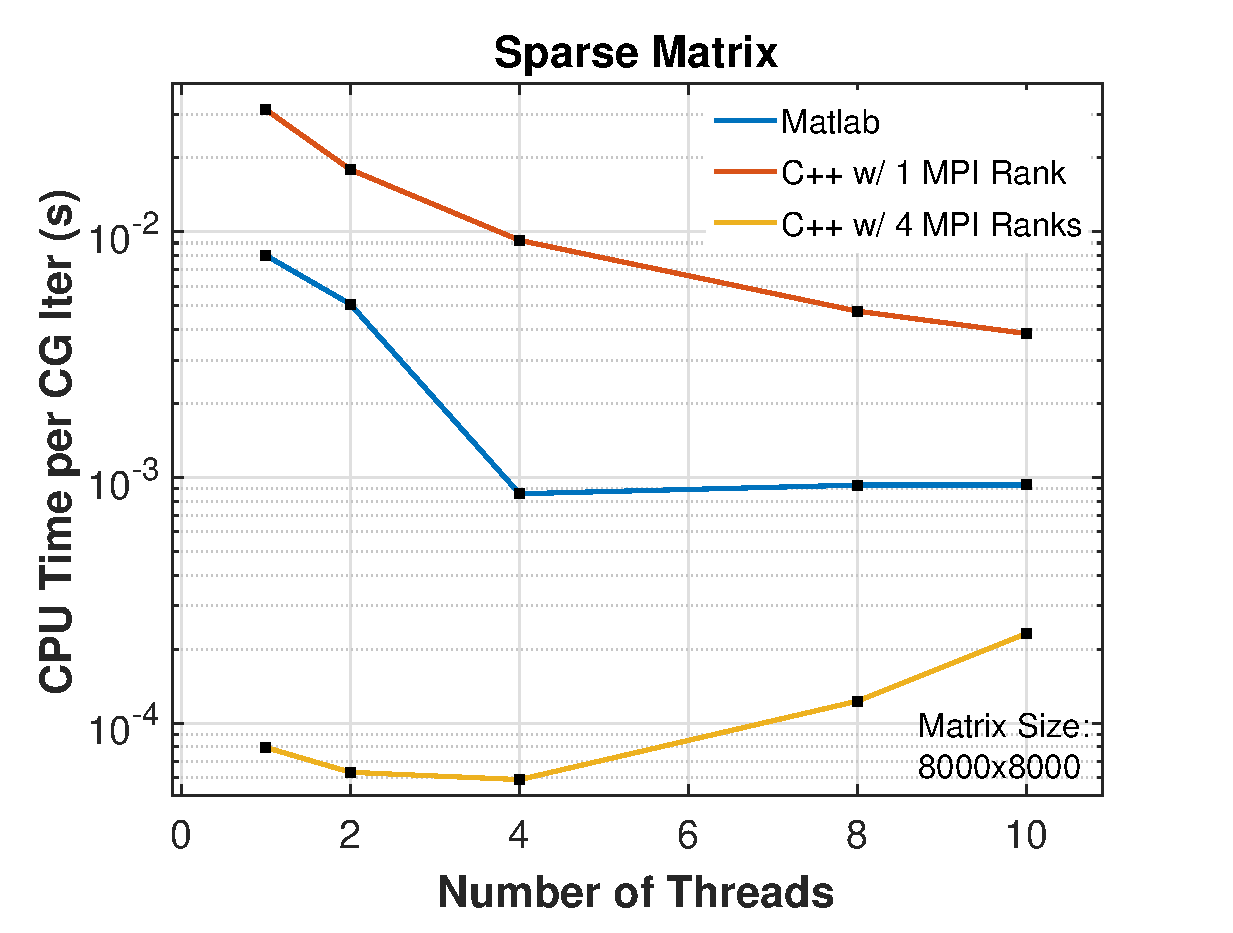
\includegraphics[width=1.0\textwidth]{sparse_matrix_benchmarks_report.eps}  
	\end{minipage}
	\caption{Benchmarks.}
	\label{fig:benchmarks}
\end{figure}



\section{Conclusions and Future work}
This study demonstrates a straightforward hybrid parallelization of the CG algorithm for solving matrix equations for both dense and sparse matrices. A substantial speedup over the serial version was achieved, especially for dense matrices. The parallelization uses a data-based approach by splitting the matrices and vectors into horizontal blocks. Using both MPI and OpenMP with a moderate number of threads provides the best performance. The scaling for dense matrices which involve many more operations is significantly better than for sparse matrices of similar size when they are stored in CRS format. However, the solution of matrices stored in CRS format is usually at least an order of magnitude faster than if the same matrix is stored in dense format. For sparse matrices, more significant speedups are expected when solving larger matrices ($>2 \cdot 10^{5}$). Neither SIMD vectorization, OpenMP tasks, nor sections yield any additional speedup. This work is applicable to areas of scientific computing where the model results in a symmetric and positive-definite matrix. An example is semiconductor device modeling which is the research field of the author. This work can be generalized for non-symmetric matrices by using the biconjugate gradient method and similar parallelization strategies may be used \cite{Ning}. Also the OpenMP parallelizations can be replaced with parallelization on GPUs through use of CUDA.

\begin{thebibliography}{4}
	%NOTE: using i.e.  \cite{name1, name2} allows to get format [1, 2] for citations.
	\bibitem{Golub} Gene H. Golub,  Charles F. Van Loan. Matrix computations (3rd ed.). “Chapter 10”, 1996
	\bibitem{Gummel} H. K. Gummel, A self-consistent iterative scheme for one-dimensional steady state transistor calculations. IEEE Transactions on Electron Devices, 11, 1964
	\bibitem{Gift} Jiebing Sun, Kanokkorn Pimcharoen, Sean R. Wagner, Phillip M. Duxbury, Pengpeng Zhang. Nanoscale imaging of dense fiber morphology and local electrical response in conductive regioregular poly(3-hexylthiophene). Organic Electronics, 15, 2014.
	\bibitem{openmp_mpi_paper} Luis F. Romero, Eva M. Ortigosa, Sergio Romero, Emilio L. Zapata. Nesting OpenMP and MPI in the Conjugate Gradient Method for Band Systems. In: Kranzlmüller D., Kacsuk P., Dongarra J. (eds) Recent Advances in Parallel Virtual Machine and Message Passing Interface. EuroPVM/MPI 2004. Lecture Notes in Computer Science, vol 3241. Springer, Berlin, Heidelberg
	\bibitem{mpi_openmp_2} Piero Lanucara, Sergio Rovida. Conjugate-Gradients Algorithms: An MPI-OpenMP Implementation on Distributed Shared Memory Systems. European Workshop on OpenMP, 1999.	
	\bibitem{Eijkhout} Victor Eijkhout. Parallel Programming in MPI and OpenMP, 2017
	\bibitem{hdf5} \url{https://www.hdfgroup.org/solutions/hdf5/}
	\bibitem{Ning} Zhao Ning, Wang XuBen. A Parallel Preconditioned Bi-Conjugate Gradient Stabilized Solver for the Poisson Problem. Journal of Computers, 7, 12, 2012.
\end{thebibliography}



\section*{Supplementary Material}   %asterisk * removes numbering
The code was compiled using the Intel 2018 compiler, OpenMPI 2.1.2, and HDF5 1.8.16. Note that to compile C++ code with HDF5, one needs to use the \texttt{h5c++} command. A make file is included in the Git repository and can be run on Unix systems with the \texttt{make} command to compile all of the code into an executable.

All code, make files, raw data, and results figures (in Matlab .fig format) can be found in the Git repository: 
\url{https://github.com/tgolubev/Conjugate_Gradient_with_MPI_and_OpenMP}.




\end{document}